% Options for packages loaded elsewhere
\PassOptionsToPackage{unicode}{hyperref}
\PassOptionsToPackage{hyphens}{url}
%
\documentclass[
  a4paper,
  portrait]{book}

\usepackage{amsmath,amssymb}
\usepackage{iftex}
\ifPDFTeX
  \usepackage[T1]{fontenc}
  \usepackage[utf8]{inputenc}
  \usepackage{textcomp} % provide euro and other symbols
\else % if luatex or xetex
  \usepackage{unicode-math}
  \defaultfontfeatures{Scale=MatchLowercase}
  \defaultfontfeatures[\rmfamily]{Ligatures=TeX,Scale=1}
\fi
\usepackage{lmodern}
\ifPDFTeX\else  
    % xetex/luatex font selection
\fi
% Use upquote if available, for straight quotes in verbatim environments
\IfFileExists{upquote.sty}{\usepackage{upquote}}{}
\IfFileExists{microtype.sty}{% use microtype if available
  \usepackage[]{microtype}
  \UseMicrotypeSet[protrusion]{basicmath} % disable protrusion for tt fonts
}{}
\makeatletter
\@ifundefined{KOMAClassName}{% if non-KOMA class
  \IfFileExists{parskip.sty}{%
    \usepackage{parskip}
  }{% else
    \setlength{\parindent}{0pt}
    \setlength{\parskip}{6pt plus 2pt minus 1pt}}
}{% if KOMA class
  \KOMAoptions{parskip=half}}
\makeatother
\usepackage{xcolor}
\setlength{\emergencystretch}{3em} % prevent overfull lines
\setcounter{secnumdepth}{5}
% Make \paragraph and \subparagraph free-standing
\ifx\paragraph\undefined\else
  \let\oldparagraph\paragraph
  \renewcommand{\paragraph}[1]{\oldparagraph{#1}\mbox{}}
\fi
\ifx\subparagraph\undefined\else
  \let\oldsubparagraph\subparagraph
  \renewcommand{\subparagraph}[1]{\oldsubparagraph{#1}\mbox{}}
\fi

\usepackage{color}
\usepackage{fancyvrb}
\newcommand{\VerbBar}{|}
\newcommand{\VERB}{\Verb[commandchars=\\\{\}]}
\DefineVerbatimEnvironment{Highlighting}{Verbatim}{commandchars=\\\{\}}
% Add ',fontsize=\small' for more characters per line
\usepackage{framed}
\definecolor{shadecolor}{RGB}{241,243,245}
\newenvironment{Shaded}{\begin{snugshade}}{\end{snugshade}}
\newcommand{\AlertTok}[1]{\textcolor[rgb]{0.68,0.00,0.00}{#1}}
\newcommand{\AnnotationTok}[1]{\textcolor[rgb]{0.37,0.37,0.37}{#1}}
\newcommand{\AttributeTok}[1]{\textcolor[rgb]{0.40,0.45,0.13}{#1}}
\newcommand{\BaseNTok}[1]{\textcolor[rgb]{0.68,0.00,0.00}{#1}}
\newcommand{\BuiltInTok}[1]{\textcolor[rgb]{0.00,0.23,0.31}{#1}}
\newcommand{\CharTok}[1]{\textcolor[rgb]{0.13,0.47,0.30}{#1}}
\newcommand{\CommentTok}[1]{\textcolor[rgb]{0.37,0.37,0.37}{#1}}
\newcommand{\CommentVarTok}[1]{\textcolor[rgb]{0.37,0.37,0.37}{\textit{#1}}}
\newcommand{\ConstantTok}[1]{\textcolor[rgb]{0.56,0.35,0.01}{#1}}
\newcommand{\ControlFlowTok}[1]{\textcolor[rgb]{0.00,0.23,0.31}{#1}}
\newcommand{\DataTypeTok}[1]{\textcolor[rgb]{0.68,0.00,0.00}{#1}}
\newcommand{\DecValTok}[1]{\textcolor[rgb]{0.68,0.00,0.00}{#1}}
\newcommand{\DocumentationTok}[1]{\textcolor[rgb]{0.37,0.37,0.37}{\textit{#1}}}
\newcommand{\ErrorTok}[1]{\textcolor[rgb]{0.68,0.00,0.00}{#1}}
\newcommand{\ExtensionTok}[1]{\textcolor[rgb]{0.00,0.23,0.31}{#1}}
\newcommand{\FloatTok}[1]{\textcolor[rgb]{0.68,0.00,0.00}{#1}}
\newcommand{\FunctionTok}[1]{\textcolor[rgb]{0.28,0.35,0.67}{#1}}
\newcommand{\ImportTok}[1]{\textcolor[rgb]{0.00,0.46,0.62}{#1}}
\newcommand{\InformationTok}[1]{\textcolor[rgb]{0.37,0.37,0.37}{#1}}
\newcommand{\KeywordTok}[1]{\textcolor[rgb]{0.00,0.23,0.31}{#1}}
\newcommand{\NormalTok}[1]{\textcolor[rgb]{0.00,0.23,0.31}{#1}}
\newcommand{\OperatorTok}[1]{\textcolor[rgb]{0.37,0.37,0.37}{#1}}
\newcommand{\OtherTok}[1]{\textcolor[rgb]{0.00,0.23,0.31}{#1}}
\newcommand{\PreprocessorTok}[1]{\textcolor[rgb]{0.68,0.00,0.00}{#1}}
\newcommand{\RegionMarkerTok}[1]{\textcolor[rgb]{0.00,0.23,0.31}{#1}}
\newcommand{\SpecialCharTok}[1]{\textcolor[rgb]{0.37,0.37,0.37}{#1}}
\newcommand{\SpecialStringTok}[1]{\textcolor[rgb]{0.13,0.47,0.30}{#1}}
\newcommand{\StringTok}[1]{\textcolor[rgb]{0.13,0.47,0.30}{#1}}
\newcommand{\VariableTok}[1]{\textcolor[rgb]{0.07,0.07,0.07}{#1}}
\newcommand{\VerbatimStringTok}[1]{\textcolor[rgb]{0.13,0.47,0.30}{#1}}
\newcommand{\WarningTok}[1]{\textcolor[rgb]{0.37,0.37,0.37}{\textit{#1}}}

\providecommand{\tightlist}{%
  \setlength{\itemsep}{0pt}\setlength{\parskip}{0pt}}\usepackage{longtable,booktabs,array}
\usepackage{calc} % for calculating minipage widths
% Correct order of tables after \paragraph or \subparagraph
\usepackage{etoolbox}
\makeatletter
\patchcmd\longtable{\par}{\if@noskipsec\mbox{}\fi\par}{}{}
\makeatother
% Allow footnotes in longtable head/foot
\IfFileExists{footnotehyper.sty}{\usepackage{footnotehyper}}{\usepackage{footnote}}
\makesavenoteenv{longtable}
\usepackage{graphicx}
\makeatletter
\def\maxwidth{\ifdim\Gin@nat@width>\linewidth\linewidth\else\Gin@nat@width\fi}
\def\maxheight{\ifdim\Gin@nat@height>\textheight\textheight\else\Gin@nat@height\fi}
\makeatother
% Scale images if necessary, so that they will not overflow the page
% margins by default, and it is still possible to overwrite the defaults
% using explicit options in \includegraphics[width, height, ...]{}
\setkeys{Gin}{width=\maxwidth,height=\maxheight,keepaspectratio}
% Set default figure placement to htbp
\makeatletter
\def\fps@figure{htbp}
\makeatother

\makeatletter
\@ifpackageloaded{bookmark}{}{\usepackage{bookmark}}
\makeatother
\makeatletter
\@ifpackageloaded{caption}{}{\usepackage{caption}}
\AtBeginDocument{%
\ifdefined\contentsname
  \renewcommand*\contentsname{Table of contents}
\else
  \newcommand\contentsname{Table of contents}
\fi
\ifdefined\listfigurename
  \renewcommand*\listfigurename{List of Figures}
\else
  \newcommand\listfigurename{List of Figures}
\fi
\ifdefined\listtablename
  \renewcommand*\listtablename{List of Tables}
\else
  \newcommand\listtablename{List of Tables}
\fi
\ifdefined\figurename
  \renewcommand*\figurename{Figure}
\else
  \newcommand\figurename{Figure}
\fi
\ifdefined\tablename
  \renewcommand*\tablename{Table}
\else
  \newcommand\tablename{Table}
\fi
}
\@ifpackageloaded{float}{}{\usepackage{float}}
\floatstyle{ruled}
\@ifundefined{c@chapter}{\newfloat{codelisting}{h}{lop}}{\newfloat{codelisting}{h}{lop}[chapter]}
\floatname{codelisting}{Listing}
\newcommand*\listoflistings{\listof{codelisting}{List of Listings}}
\makeatother
\makeatletter
\makeatother
\makeatletter
\@ifpackageloaded{caption}{}{\usepackage{caption}}
\@ifpackageloaded{subcaption}{}{\usepackage{subcaption}}
\makeatother
\ifLuaTeX
  \usepackage{selnolig}  % disable illegal ligatures
\fi
\usepackage{bookmark}

\IfFileExists{xurl.sty}{\usepackage{xurl}}{} % add URL line breaks if available
\urlstyle{same} % disable monospaced font for URLs
\hypersetup{
  pdftitle={Die Tafelstube},
  pdfauthor={Lena-Marie Hoppe},
  hidelinks,
  pdfcreator={LaTeX via pandoc}}

\title{Die Tafelstube}
\author{Lena-Marie Hoppe}
\date{2024-06-14}

\begin{document}
\frontmatter
\maketitle

\renewcommand*\contentsname{Table of contents}
{
\setcounter{tocdepth}{2}
\tableofcontents
}
\mainmatter
\bookmarksetup{startatroot}

\chapter{Katalog zur Ausstellung: Die
Tafelstube}\label{katalog-zur-ausstellung-die-tafelstube}

Ein Katalog mit Kunstwerken aus der CbDD-Sammlung. Textteil:
\href{https://www.deckenmalerei.eu/42d06165-58e7-4653-bfe4-3d5f7091fc33\#6e73f774-4b7f-4e37-937b-e11cc35c5bc8}{6e73f774-4b7f-4e37-937b-e11cc35c5bc8}

Die Tafelstube (Belagerungsszenen des Langen Türkenkriegs an der Decke)
{[}Raum{]}

This work is licensed under a Creative Commons
Attribution-NonCommercial-NoDerivs 4.0 International License.

\bookmarksetup{startatroot}

\chapter{Die Tafelstube}\label{die-tafelstube}

\textbf{How to use your own text for processing}

\begin{enumerate}
\def\labelenumi{\arabic{enumi}.}
\tightlist
\item
  Add a new Text item to the wikibase.
  \href{https://computational-publishing-service.wikibase.cloud/wiki/Special:NewItem}{link
  to wikibase new item} the item should contain the following
  statements:
\end{enumerate}

\begin{itemize}
\tightlist
\item
  P57 (external link): link to the html file containing the new text
\item
  P46 (kurator): Item of the curator. you may use an existing item like
  Q210 (Ulrike seeger) for test purposes
\item
  P53 (license): Item of a license for the text. e.g Q203 (CC BY-NC-ND
  4.0 DEED )
\item
  P6 (is part of): set value to Q218 (Schlossanlage Weikersheim)
\end{itemize}

\begin{enumerate}
\def\labelenumi{\arabic{enumi}.}
\setcounter{enumi}{1}
\item
  check if your new text item occurs in the list of selected text items:
  \href{https://computational-publishing-service.wikibase.cloud/query/\#PREFIX\%20cps\%3A\%20\%3Chttps\%3A\%2F\%2Fcomputational-publishing-service.wikibase.cloud\%2Fentity\%2F\%3E\%0APREFIX\%20cpss\%3A\%20\%3Chttps\%3A\%2F\%2Fcomputational-publishing-service.wikibase.cloud\%2Fentity\%2Fstatement\%2F\%3E\%0APREFIX\%20cpsv\%3A\%20\%3Chttps\%3A\%2F\%2Fcomputational-publishing-service.wikibase.cloud\%2Fvalue\%2F\%3E\%0APREFIX\%20cpspt\%3A\%20\%3Chttps\%3A\%2F\%2Fcomputational-publishing-service.wikibase.cloud\%2Fprop\%2Fdirect\%2F\%3E\%0APREFIX\%20cpsp\%3A\%20\%3Chttps\%3A\%2F\%2Fcomputational-publishing-service.wikibase.cloud\%2Fprop\%2F\%3E\%0APREFIX\%20cpsps\%3A\%20\%3Chttps\%3A\%2F\%2Fcomputational-publishing-service.wikibase.cloud\%2Fprop\%2Fstatement\%2F\%3E\%0APREFIX\%20cpspq\%3A\%20\%3Chttps\%3A\%2F\%2Fcomputational-publishing-service.wikibase.cloud\%2Fprop\%2Fqualifier\%2F\%3E\%0A\%0ASELECT\%20\%3FtextItem\%20\%3FkuratorLabel\%20\%3FtextUrl\%0AWHERE\%0A\%7B\%0A\%20\%20\%3FtextItem\%20cpsp\%3AP46\%20\%3FkuratorStatement.\%20\%0A\%20\%20\%3FkuratorStatement\%20cpsps\%3AP46\%20\%3FkuratorItem.\%20\%0A\%20\%20\%3FkuratorItem\%20rdfs\%3Alabel\%20\%3FkuratorLabel.\%0A\%20\%20\%3FtextItem\%20cpsp\%3AP57\%20\%3Furlstatement.\%20\%0A\%20\%20\%3Furlstatement\%20cpsps\%3AP57\%20\%3FtextUrl.\%20\%0A\%7D}{Link
  to wikibase query service}
\item
  set parameter of get\_text() to the id of your new text item e.g.:
  get\_text(``Q209'')
\end{enumerate}

\begin{Shaded}
\begin{Highlighting}[]
\NormalTok{get\_text(}\StringTok{"Q232"}\NormalTok{)}
\CommentTok{\#Text zur Tafelstube}
\end{Highlighting}
\end{Shaded}

Wikibase link:
\url{https://computational-publishing-service.wikibase.cloud/entity/Q232}

Kurator: Seeger, Ulrike

Die Tafelstube

Beschreibung

\xc3\x96stlich an den Rittersaal schlie\xc3\x9ft ein gro\xc3\x9fer, 1837
unterteilter Raum an, bei dem es sich um die einstige Tafelstube
handelt.{[}1{]} Als Eckraum mit vier Doppelfenstern zur Gartenseite und
weiteren drei Doppelfenstern zur Grabenseite erhielt die Tafelstube viel
Licht. Auch konnte der F\xc3\xbcrst von dort aus auf die Stadt und den
Lustgarten blicken, der in der Renaissance dem Schloss
s\xc3\xbcd\xc3\xb6stlich vorgelagert war.{[}2{]} Gemessen an der
Gr\xc3\xb6\xc3\x9fe des Raumes war die Tafelstube nicht sehr hoch. Die
Decke mit kr\xc3\xa4ftigen Unterz\xc3\xbcgen ruhte
urspr\xc3\xbcnglich auf vier St\xc3\xbctzen, deren Position einem Plan
des 19. Jahrhunderts zu entnehmen ist. Die Fensternischen waren in
Fortsetzung der Saaldekoration mit Roll- und Beschlagwerk stuckiert,
wof\xc3\xbcr Christoph Limmerich in Frage kommt, der auch im Saal
gearbeitet hat.

Logistisch geh\xc3\xb6ren zur Tafelstube zwei Service-Kabinetten
beiderseits des Durchgangs zwischen Saal und Tafelstube. Sie haben eine
geringe Raumh\xc3\xb6he, da \xc3\xbcber ihnen und dem Durchgang die
Empore an der Ostseite des Saals verl\xc3\xa4uft. Das Kabinett der
Gartenseite war von der Tafelstube und vom Durchgang aus
zug\xc3\xa4nglich, das Kabinett der Hofseite au\xc3\x9fer von der
Tafelstube vom Altan aus. Der Altan entlang der Hofseite des Saalbaus
verband das hofseitige Kabinett mit der K\xc3\xbcche im Erdgeschoss des
K\xc3\xbcchenbaus, sodass bevorzugt dieses Kabinett dem Anrichten der
Speisen gedient haben d\xc3\xbcrfte. Dank der Verbindung zu dem ja erst
in einem zweiten Bauabschnitt errichteten Altan, blieb der Rittersaal
vom Transport der Speisen verschont.

Der repr\xc3\xa4sentative Zugang zur Tafelstube erfolgte vom Saal aus,
wo der Besucher das imposante Portal mit der Belagerung von Gran
(Eszergom) im Hintergrund einer wilden T\xc3\xbcrkenschlacht,
bekr\xc3\xb6nt von der Skulptur des heiligen Georg zu durchschreiten
hatte. Ein zweiter Zugang bestand oder lie\xc3\x9f sich zumindest
einrichten von der geradel\xc3\xa4ufigen Treppe im sp\xc3\xa4teren
Langenburger Bau.

Die urspr\xc3\xbcngliche Bezeichnung des Raumes und seine Ausstattung

Im Inventar von 1625\xe2\x80\x9327 wurde der Raum im Anschluss an den
Saal als \xe2\x80\x9eSaalstube\xe2\x80\x9c bezeichnet.{[}3{]} Die
W\xc3\xa4nde waren mit 14 Ledertapeten beschlagen. Im Raum standen zwei
l\xc3\xa4ngsrechtecke Tische, ein quadratischer Tisch und eine
\xe2\x80\x9egro\xc3\x9fe Landtafel\xe2\x80\x9c sowie 31 Sessel mit
Lederbez\xc3\xbcgen und goldenem Dekor.{[}4{]} Im Schadensinventar von
1639 wurde der Raum sodann als \xe2\x80\x9eGro\xc3\x9fe
Tafelstube\xe2\x80\x9c gef\xc3\xbchrt.{[}5{]}

{[}1{]} Die Jahreszahl der Unterteilung: Merten, Weikersheim, o. J., S.
40; Fandrey, Weikersheim, 2010, S. 51.

{[}2{]} M\xc3\xbcnzenmayer/Elfgang, Schlossgarten, 1999, Abb. S. 5.

{[}3{]} Die Kenntnis dieses Inventars verdankt die Autorin Dinah
Rottsch\xc3\xa4fer.

{[}4{]} Ebd.

{[}5{]} HZAN La 130 B\xc3\xbc 152, Schadensinventar von 1639. Die
Kenntnis und die Transkription dieser Archivalie verdankt die Autorin
Frieder Leipold. Zur Herausbildung der Tafelstube im deutschen
Schlossbau der Renaissance: Hoppe, Tafelstube, 2007
(https://adw-goe.de/en/digital-library/hoefe-und-residenzen-im-spaetmittelalterlichen-reich/gsn/rf15\_II\_121207-196/?tx\_find\_find\%5BunderlyingQuery\%5D\%5Bq\%5D\%5Bdefault\%5D=tafelstube\&tx\_find\_find\%5BunderlyingQuery\%5D\%5Bposition\%5D=1)

Programm und Synthese der einstigen Tafelstube

Tafelstube und Saal h\xc3\xa4ngen konzeptionell eng zusammen.
W\xc3\xa4hrend der Saal mit der guten Herrschaft des Grafen Wolfgang
einen regionalen Radius beschreibt, weitet sich in der Tafelstube der
Horizont auf den Beitrag der Grafschaft Hohenlohe zur Rettung der
Christenheit vor osmanischer Herrschaft. R\xc3\xa4umlich
verkn\xc3\xbcpft sind die beiden Bildprogramme durch das Relief des
Innenportals mit der Belagerung von Gran (Eszergom) 1594 und die
Deckenmalerei des Durchgangs, die mit der Beweinung des toten Adonis
durch Venus und Amor auf den tragischen Tod des j\xc3\xbcngsten Sohnes
bei der Belagerung von Gran (Eszergom) 1604 vorausweist. Adonis als
passionierter J\xc3\xa4ger wiederum verband die Tafelstube mit dem
Jagdzyklus an der Decke des Saals.

\textbf{How to select images for processing}

Images are selected via the sparql query. The method get\_img() is
capable of using a wikibase item id as parameter to select images with
the property P6 (is part of) linking to the given item id.

\begin{enumerate}
\def\labelenumi{\arabic{enumi}.}
\item
  select a valid location id from the query result:
  \href{https://computational-publishing-service.wikibase.cloud/query/\#PREFIX\%20cps\%3A\%20\%3Chttps\%3A\%2F\%2Fcomputational-publishing-service.wikibase.cloud\%2Fentity\%2F\%3E\%0APREFIX\%20cpss\%3A\%20\%3Chttps\%3A\%2F\%2Fcomputational-publishing-service.wikibase.cloud\%2Fentity\%2Fstatement\%2F\%3E\%0APREFIX\%20cpsv\%3A\%20\%3Chttps\%3A\%2F\%2Fcomputational-publishing-service.wikibase.cloud\%2Fvalue\%2F\%3E\%0APREFIX\%20cpspt\%3A\%20\%3Chttps\%3A\%2F\%2Fcomputational-publishing-service.wikibase.cloud\%2Fprop\%2Fdirect\%2F\%3E\%0APREFIX\%20cpsp\%3A\%20\%3Chttps\%3A\%2F\%2Fcomputational-publishing-service.wikibase.cloud\%2Fprop\%2F\%3E\%0APREFIX\%20cpsps\%3A\%20\%3Chttps\%3A\%2F\%2Fcomputational-publishing-service.wikibase.cloud\%2Fprop\%2Fstatement\%2F\%3E\%0APREFIX\%20cpspq\%3A\%20\%3Chttps\%3A\%2F\%2Fcomputational-publishing-service.wikibase.cloud\%2Fprop\%2Fqualifier\%2F\%3E\%0A\%0ASELECT\%20DISTINCT\%20\%3FpartOfItem\%20\%3FpartOfItemLabel\%0AWHERE\%0A\%7B\%0A\%20\%20\%3FimgItem\%20cpsp\%3AP107\%20\%3FurlStatement.\%20\%0A\%20\%20\%3FurlStatement\%20cpsps\%3AP107\%20\%3FimgUrl.\%20\%0A\%20\%20\%3FimgItem\%20cpsp\%3AP60\%20\%3FdateStatement.\%20\%0A\%20\%20\%3FdateStatement\%20cpsps\%3AP60\%20\%3FpublishDate.\%20\%0A\%20\%20\%3FimgItem\%20cpsp\%3AP6\%20\%3FpartOfStatement.\%0A\%20\%20\%3FpartOfStatement\%20cpsps\%3AP6\%20\%3FpartOfItem.\%0A\%20\%20SERVICE\%20wikibase\%3Alabel\%20\%7B\%0A\%20\%20\%20\%20\%20\%20bd\%3AserviceParam\%20wikibase\%3Alanguage\%20\%22de\%2Cen\%22.\%0A\%20\%20\%20\%20\%20\%20\%3FpartOfItem\%20rdfs\%3Alabel\%20\%3FpartOfItemLabel.\%0A\%20\%20\%20\%20\%20\%20\%3FpartOfItem\%20schema\%3Adescription\%20\%3FpartOfItemDescr.\%0A\%20\%20\%20\%20\%7D\%0A\%7D\%20GROUP\%20BY\%20\%3FpartOfItem\%20\%3FpartOfItemLabel}{Link
  to wikibase query service}
\item
  set parameter of get\_img() to the id of your selected location item
  e.g.: get\_img(``Q217'')
\end{enumerate}

\begin{Shaded}
\begin{Highlighting}[]
\NormalTok{get\_img(}\StringTok{"Q231"}\NormalTok{)}
\CommentTok{\#Bild Tafelstube}
\end{Highlighting}
\end{Shaded}

Wikibase link:
\url{https://computational-publishing-service.wikibase.cloud/entity/Q234}

Title: Einstige Tafelstube \& Raum 69a -- nach Südosten

Year: 2018

Description: Wolfgang Beringer, Baumeister und Steinmetz - Georg Stegle,
Baumeister - Entwurf: Georges Robin, Architekt - Elias Gunzenhäuser,
Zimmermann - Weikersheim, Marktplatz 11 - ab 1595

Wikibase link:
\url{https://computational-publishing-service.wikibase.cloud/entity/Q234}

Title: Einstige Tafelstube \& Raum 69a -- nach Südosten

Year: 2018-01-01T00:00:00Z

Description: Wolfgang Beringer, Baumeister und Steinmetz - Georg Stegle,
Baumeister - Entwurf: Georges Robin, Architekt - Elias Gunzenhäuser,
Zimmermann - Weikersheim, Marktplatz 11 - ab 1595

\includegraphics{tafelstube_files/figure-pdf/cell-3-output-2.png}
\includegraphics{tafelstube_files/figure-pdf/cell-3-output-3.png}

\begin{Shaded}
\begin{Highlighting}[]
\NormalTok{get\_text(}\StringTok{"Q264"}\NormalTok{)}
\CommentTok{\#Programm und Synthese der einstigen Tafelstube}
\end{Highlighting}
\end{Shaded}

Wikibase link:
\url{https://computational-publishing-service.wikibase.cloud/entity/Q264}

Kurator: Seeger, Ulrike

Programm und Synthese der einstigen Tafelstube

Tafelstube und Saal h\xc3\xa4ngen konzeptionell eng zusammen.
W\xc3\xa4hrend der Saal mit der guten Herrschaft des Grafen Wolfgang
einen regionalen Radius beschreibt, weitet sich in der Tafelstube der
Horizont auf den Beitrag der Grafschaft Hohenlohe zur Rettung der
Christenheit vor osmanischer Herrschaft. R\xc3\xa4umlich
verkn\xc3\xbcpft sind die beiden Bildprogramme durch das Relief des
Innenportals mit der Belagerung von Gran (Eszergom) 1594 und die
Deckenmalerei des Durchgangs, die mit der Beweinung des toten Adonis
durch Venus und Amor auf den tragischen Tod des j\xc3\xbcngsten Sohnes
bei der Belagerung von Gran (Eszergom) 1604 vorausweist. Adonis als
passionierter J\xc3\xa4ger wiederum verband die Tafelstube mit dem
Jagdzyklus an der Decke des Saals.

\begin{Shaded}
\begin{Highlighting}[]
\NormalTok{get\_graph()}
\end{Highlighting}
\end{Shaded}

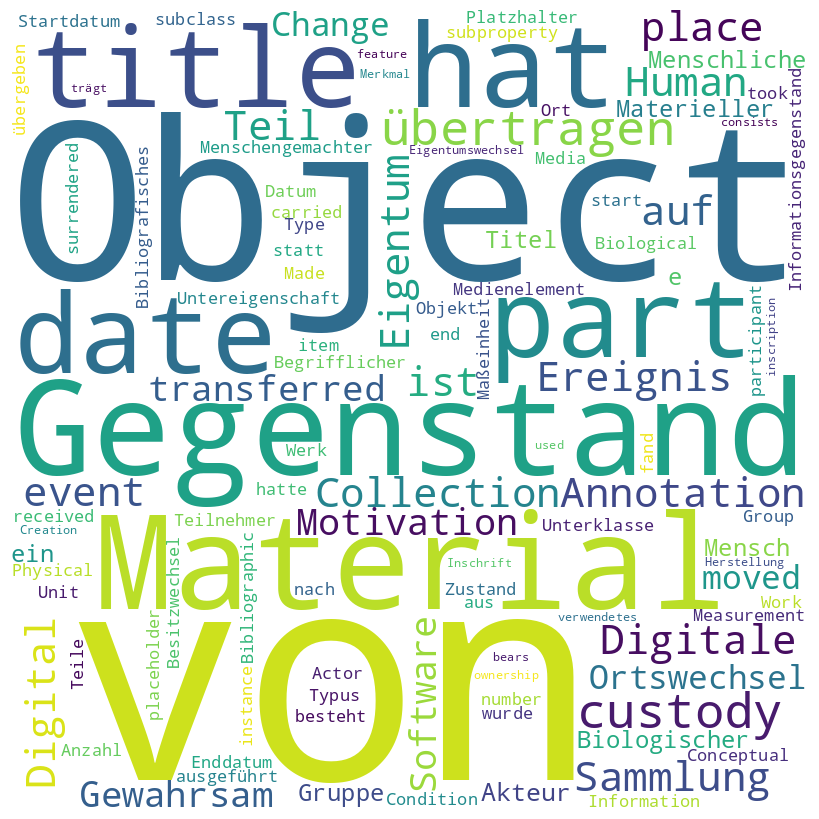
\includegraphics{tafelstube_files/figure-pdf/cell-5-output-1.png}

\part{Belagerungsszenen des Langen Türkenkriegs an der Decke}

\begin{Shaded}
\begin{Highlighting}[]
\ImportTok{from}\NormalTok{ funktionen }\ImportTok{import} \OperatorTok{*}
\end{Highlighting}
\end{Shaded}

\begin{Shaded}
\begin{Highlighting}[]
\NormalTok{get\_text(}\StringTok{"Q278"}\NormalTok{)}
\CommentTok{\#Belagerungsszenen des Langen Türkenkrieges}
\end{Highlighting}
\end{Shaded}

Wikibase link:
\url{https://computational-publishing-service.wikibase.cloud/entity/Q278}

Kurator: Seeger, Ulrike

Belagerungsszenen des Langen T\xc3\xbcrkenkriegs an der Decke

Zuweisung der Gem\xc3\xa4lde in die einstige Tafelstube

Die einstige Deckenzier der Tafelstube ist den Inventaren, die ja
lediglich die mobilen Einrichtungsgegenst\xc3\xa4nde auff\xc3\xbchren,
nicht zu entnehmen. Einer Haustradition von Schloss Weikersheim zufolge
waren an der Decke urspr\xc3\xbcnglich jene 12 gro\xc3\x9fformatigen
Belagerungsszenen angebracht, die sich heute in musealer Aufstellung
teilweise im Flur vor dem einstigen Appartement Graf Wolfgangs im
K\xc3\xbcchenbau befinden.{[}1{]} Bei der Unterteilung des Raumes 1837
wurden sie abgenommen und tauchten im Schloss 1946 wieder auf.{[}2{]}
Ihre Anzahl, ihre Aufteilung in vier schmale und acht breite Bilder
sowie wie die exakten Ma\xc3\x9fe{[}3{]} passen sehr gut zu den Gefachen
der Balkendecke. Es besteht also kein Anlass, an dieser Haustradition zu
zweifeln.

Urheberschaft und Datierung der Gem\xc3\xa4lde

Nahezu alle Gem\xc3\xa4lde sind stilistisch Balthasar Katzenberger
zuzuschreiben. Ein Vertrag wie der zu den Deckengem\xc3\xa4lden des
Rittersaals hat sich nicht erhalten, sodass sie nicht genau datiert
sind. Sie entstanden jedoch vermutlich sofort im Anschluss an die im
November 1602 quittierten Deckengem\xc3\xa4lde des Saals, also von 1603
bis 1604. Bei der sp\xc3\xa4testen dargestellten Belagerung von 1604
handelt es sich um einen Nachz\xc3\xbcgler. Ihr Duktus ist nicht der von
Katzenberger, was sich insbesondere an den Wolkenformationen zeigt, die
entgegen Katzenbergers Gepflogenheit wei\xc3\x9f konturiert sind.
M\xc3\xb6glicherweise ersetzte das Gem\xc3\xa4lde ein anderes Bild und
wurde zu einem Zeitpunkt gew\xc3\xbcnscht, als Katzenberger nicht zur
Verf\xc3\xbcgung stand. Der Anlass f\xc3\xbcr die nachtr\xc3\xa4gliche
Bestellung war der Tod von Graf Ludwig Kasimir bei der dargestellten
Belagerung von Gran im Jahr 1604, an die das Gem\xc3\xa4lde erinnert.

Komposition und Darstellungsmodus der Gem\xc3\xa4lde

Die hochrechteckigen Belagerungsszenen folgen im Aufbau prinzipiell den
achteckigen Jagdgem\xc3\xa4lden im Saal. Im Vordergrund hat Katzenberger
ein Get\xc3\xbcmmel inszeniert, das sich am unteren Bildrand abspielt
und dessen Protagonisten von beiden Seiten ins Bild reiten oder treten.
Seitlich wird das Geschehen von hohen Repoussoir-B\xc3\xa4ume gerahmt,
die sich am oberen Bildrand durch die Beschriftung der Gem\xc3\xa4lde
mit dunklen Buchstaben vor blauem Himmel zu einer ovalen Rahmung
zusammenschlie\xc3\x9fen. Im Mittel- und Hintergrund schilderte
Katzenberger in weitl\xc3\xa4ufiger Landschaft die Belagerung einer
Festung. Rings um die Festung stehen die Zelte der Belagerer,
entz\xc3\xbcnden sich Scharm\xc3\xbctzel und hin und wieder auch
kleinere Schlachten.

Thema, Vorlagen, Auswahl und Konzeption des Zyklus

Die Gem\xc3\xa4lde zeigen Belagerungen ungarischer Festungen, die sich
w\xc3\xa4hrend des Langen T\xc3\xbcrkenkriegs ergaben. Der Lange
T\xc3\xbcrkenkrieg begann 1593 zwischen dem Osmanischen Reich und den
Habsburgern nachdem es schon vorher auf beiden Seiten zu
Grenzverletzungen gekommen war.{[}4{]} Es handelte sich um einen
Festungskrieg, bei dem die im Anschluss an die osmanische Belagerung
Wiens im Jahr 1529 auf beiden Seiten ausgebauten Festungen wechselseitig
belagert wurden. Beendet wurde der Krieg erst 1606 mit dem Frieden von
Zsitvatorok. Die in Weikersheim dargestellten Belagerungen beginnen
angeblich schon 1590, sp\xc3\xa4testens jedoch 1594 und reichen bis in
das Jahr 1604.

Der Lange T\xc3\xbcrkenkrieg mit seinen vielen Belagerungen bestimmte
bereits das das Programm des inneren Ostportals des Rittersaals. Dieses
Portal f\xc3\xbchrte nach Ansicht der Autorin nicht von der Tafelstube
in den Saal, sondern vom Saal in die Tafelstube. Es bereitete den
Besucher des Saals thematisch auf das Bildprogramm der Tafelstube vor,
zumal das Portal und die Deckengem\xc3\xa4lde der Tafelstube zur
gleichen Zeit entstanden. Der Stuckateur Gerhard Schmidt schuf sein 1603
signiertes und datiertes Portal im Saal, w\xc3\xa4hrend Katzenberger
seine Gem\xc3\xa4lde in der Werkstatt malte.

Als Vorlagen f\xc3\xbcr die Belagerungsszenen im Hintergrund dienten
Kupferstiche, die einer ausf\xc3\xbchrlichen, 1602 in
N\xc3\xbcrnberg erschienenen Chronik \xc3\xbcber den
T\xc3\xbcrkenkrieg beigebunden waren.{[}5{]} Verfasser des Werkes
\xe2\x80\x9eChronologia oder Historische Beschreibung aller
Kriegsemporungen und Bel\xc3\xa4gerungen der St\xc3\xa4tt und Vestungen,
auch Scharm\xc3\xbctzeln und Schlachten, so in Ober- und Under-Ungarn,
auch Sibenb\xc3\xbcrgen, mit dem T\xc3\xbcrcken von A. 1395 bi\xc3\x9f
auff gegenwertige Zeit gedenckhw\xc3\xbcrdig geschehen
\xe2\x80\xa6\xe2\x80\x9c{[}6{]} war Hieronymus Oertl (Ortelius), der in
Wien als kaiserlicher Notar wegen seiner protestantischen Gesinnung 1580
in Ungnade gefallen war und sich danach in
N\xc3\xbcrnberg niederlie\xc3\x9f.{[}7{]} Die Anregung zu dem Werk ging
von seinem Schwager, dem N\xc3\xbcrnberger Kupferstecher und Verleger
Johann Sibmacher aus. Sibmacher zeichnete die Belagerungsszenen nach
Ortelius Vorgaben und stach sie in Kupfer.{[}8{]}

Die insgesamt 28 Kupfer wurden in der deutschsprachigen Legende in ihrem
Sujet genau benannt und mit dem Jahr der Belagerung versehen.
Katzenberger \xc3\xbcbernahm diese Beischriften buchstabengetreu
f\xc3\xbcr seine Deckengem\xc3\xa4lde. Aufgrund der sehr genauen
\xc3\x9cbernahmen in Wort und Bild kann man davon ausgehen, dass
Ortelius\xe2\x80\x98 Chronik Graf Wolfgang im Jahr ihres Erscheinens
1602 vorlag. Ausgew\xc3\xa4hlt aus den 28 Kupfern wurden
Belagerungsaktionen sowohl der Kaiserlichen als auch der Osmanen. Harald
Dr\xc3\xb6s, der sich bislang am ausf\xc3\xbchrlichsten mit den
Weikersheimer Belagerungsszenen auseinandergesetzt hat und dem wertvolle
Hinweise zu verdanken sind,{[}9{]} vermutete deshalb sicher zurecht,
dass die Auswahl der Szenen davon bestimmt war, dass Mitglieder des
Hauses Hohenlohe beteiligt waren. Die folgende Beschreibung der Bilder
best\xc3\xa4tigt diese Vermutung. Die sp\xc3\xa4teste dargestellte
Belagerung von Gran (Eszergom), bei der der Sohn Ludwig Kasimir zu Tode
kam,{[}10{]} bezieht sich als ein Art Memorialbild auf dessen Tod. Auch
dieses tragische Ereignis wurde dem Besucher schon angek\xc3\xbcndigt,
indem im Durchgang zwischen Saal und Tafelstube die Beweinung des toten
Adonis durch Venus und Amor dargestellt wurde.

Drei der in Weikersheim dargestellten Belagerungen lagen sp\xc3\xa4ter
als das Erscheinungsjahr der Chronik. Sie wurden hinzuerfunden und
weisen deutliche Schw\xc3\xa4chen in der Schilderung des Hintergrunds
auf. Die drei jeweils an der Donau stattgefundenen Aktionen wurden aus
Landkarten und Belagerungen Sibmachers
versatzst\xc3\xbcckhaft kompiliert. Da die Gem\xc3\xa4lde keinerlei
Anhaltspunkte zu ihrer urspr\xc3\xbcnglichen Anordnung preisgeben, folgt
ihre nachfolgende Nummerierung der Chronologie der dargestellten
Belagerungen. Sie findet sich in der gleichen Reihenfolge zusammen mit
den genauen Ma\xc3\x9fen bei Harald Dr\xc3\xb6s im Band der Inschriften
des ehemaligen Landkreises Mergentheim.{[}11{]}

Rekonstruktion der einstigen Anordnung

Bei der Rekonstruktion der Decke, die Jan Lutteroth miterarbeitet und
graphisch umgesetzt hat, wurde die Reihenfolge der durch keinerlei Bild-
oder Schriftquellen \xc3\xbcberlieferten Anbringung ebenfalls
gem\xc3\xa4\xc3\x9f der Chronologie gew\xc3\xa4hlt. Die Geschichte
beginnt in angenommener Leserichtung von links nach rechts
f\xc3\xbcr den Eintretenden links oben mit dem geheimnisvollen Nachtbild
der Belagerung von Totis im Jahr 1590 (Belagerung I). Bei der
Rekonstruktion der in vier Register \xc3\xbcbereinanderliegenden Szenen
musste lediglich im dritten Register einmal die Chronologie verlassen
werden, da die Belagerung der Stadt Waitzen im Jahr 1597 (Belagerung
VII) als schmales Bildformat nicht links au\xc3\x9fen, sondern erst in
der Mitte platziert werden konnte. Sie wird nun von den Belagerungen von
Raab 1598, wiederum einem effektvollen Nachtbild (Belagerung VIII), und
der Belagerung von Ofen ebenfalls im Jahr 1598 (Belagerung IX)
flankiert.

Die drei Belagerungen, an denen S\xc3\xb6hne teilgenommen hatten
(Belagerung X, XI, XII) stehen bei der gew\xc3\xa4hlten Anordnung am
Ende der Tafelstube. Die drei darunterliegenden Fenster er\xc3\xb6ffnen
den Blick auf die Stadt s\xc3\xbcdlich des Marktplatzes. Das besonders
wichtige Gem\xc3\xa4lde mit dem bei der Belagerung von Gran (Eszergom)
1604 get\xc3\xb6teten Ludwig Kasimir (Belagerung XII) kommt als letztes
der Reihe rechts oben so zu stehen, dass Ludwig Kasimir mit seinem Pferd
Richtung Kirche reitet, wo er beigesetzt wurde. Der trauernden
Gr\xc3\xa4fin w\xc3\xbcrde auf dem Gem\xc3\xa4lde ebenfalls der Weg zur
Kirche gewiesen.

{[}1{]} Merten, Weikersheim, o. J., S. 40. Trentin-Meyer, Georg
Friedrich von Hohenlohe, 2019, S. 90 spricht versehentlich von 13
Gem\xc3\xa4lden.

{[}2{]} Freeden, Kamin, 1950, S. 142.

{[}3{]} Die Ma\xc3\x9fe bei Dr\xc3\xb6s, Inschriften Mergentheim, 2002,
S. 248. Ebd., S. 249 die bislang
ausf\xc3\xbchrlichste Auseinandersetzung mit den Gem\xc3\xa4lden.

{[}4{]} Zum Langen T\xc3\xbcrkenkrieg: Niederkorn, Langer
T\xc3\xbcrkenkrieg, 1993.

{[}5{]} Diese wichtige Vorlage bereits bei Fandrey, Weikersheim, 2010,
S. 60.

{[}6{]} Ortelius, Chronologia, 1602.

{[}7{]} Mummenhoff, Ernst, ``Oertl, Hieronymus'' in: Allgemeine Deutsche
Biographie 24 (1887), S. 445-446 {[}Online-Version{]}; URL:
https://www.deutsche-biographie.de/pnd128534958.html\#adbcontent.

{[}8{]} Ebd. Au\xc3\x9ferdem Ortelius, Chronologia, 1602, \xe2\x80\x9eAd
Lectorem\xe2\x80\x9c.

{[}9{]} Dr\xc3\xb6s, Inschriften Mergentheim, 2002, S.
248\xe2\x80\x93249.

{[}10{]} Dr\xc3\xb6s, Inschriften Mergentheim, 2002, S.
248\xe2\x80\x93250.

{[}11{]} Dr\xc3\xb6s, Inschriften Mergentheim, 2002, Nr. 366.

\chapter{Belagerungsszene I: Eroberung der Festung
Tottis}\label{belagerungsszene-i-eroberung-der-festung-tottis}

\begin{Shaded}
\begin{Highlighting}[]
\ImportTok{from}\NormalTok{ funktionen }\ImportTok{import} \OperatorTok{*}
\end{Highlighting}
\end{Shaded}

\begin{Shaded}
\begin{Highlighting}[]
\NormalTok{get\_text(}\StringTok{"Q252"}\NormalTok{)}
\CommentTok{\#Belagerungsszene I}

\NormalTok{get\_img(}\StringTok{"Q238"}\NormalTok{)}
\CommentTok{\#Vestung Tottis}
\end{Highlighting}
\end{Shaded}

Wikibase link:
\url{https://computational-publishing-service.wikibase.cloud/entity/Q252}

Kurator: Seeger, Ulrike

Belagerung I: \xe2\x80\x9eVestung Tottis, wie die von den Christen bei
der Nacht erobert worden, 1590\xe2\x80\x9c

Breites Format. Vorne rechts ins Bild hineinreitende Reiter mit
gro\xc3\x9fen Fahnen. Im Hintergrund die ungarische Festung Totis (Tata)
nach dem Vorbild von Sibmachers Kupferstich, der allerdings eine
Eroberung durch die Christen aus dem Jahr 1597 wiedergibt. Die sehr
dunkle Szenerie wird von zwei Laternen sp\xc3\xa4rlich erleuchtet. Da
Totis nicht 1590, sondern 1597 und 1598 durch die Christen erobert
wurde, und zudem zu den zeitlich als n\xc3\xa4chste dargestellten
Belagerungen eine Zeitspanne von vier Jahren liegt, kann es gut sein,
dass der Jahreszahl 1590 ein Versehen zugrunde liegt.

Wikibase link:
\url{https://computational-publishing-service.wikibase.cloud/entity/Q265}

Title: Eroberung der Festung Tottis -- Gesamtansicht

Year: 2018

Description: Teil von: Wanddekoration des Flurs \& Raum 73a
Belagerungsszenen und Türkenschlachten; Balthasar Kazenberger, Maler -
Weikersheim, Schloss Weikersheim, Flur \& Raum 73a - 1603-1604

Wikibase link:
\url{https://computational-publishing-service.wikibase.cloud/entity/Q265}

Title: Eroberung der Festung Tottis -- Gesamtansicht

Year: 2018-01-01T00:00:00Z

Description: Teil von: Wanddekoration des Flurs \& Raum 73a
Belagerungsszenen und Türkenschlachten; Balthasar Kazenberger, Maler -
Weikersheim, Schloss Weikersheim, Flur \& Raum 73a - 1603-1604

\includegraphics{belagerung_01_files/figure-pdf/cell-3-output-2.png}
\includegraphics{belagerung_01_files/figure-pdf/cell-3-output-3.png}

\chapter{Belagerungsszene II: Belagerung der Festung
Gran}\label{belagerungsszene-ii-belagerung-der-festung-gran}

\begin{Shaded}
\begin{Highlighting}[]
\ImportTok{from}\NormalTok{ funktionen }\ImportTok{import} \OperatorTok{*}
\end{Highlighting}
\end{Shaded}

\begin{Shaded}
\begin{Highlighting}[]
\NormalTok{get\_text(}\StringTok{"Q253"}\NormalTok{)}
\CommentTok{\#Belagerung II}

\NormalTok{get\_img(}\StringTok{"Q239"}\NormalTok{)}
\CommentTok{\#Festung Gran}
\end{Highlighting}
\end{Shaded}

Wikibase link:
\url{https://computational-publishing-service.wikibase.cloud/entity/Q253}

Kurator: Seeger, Ulrike

Belagerung II: \xe2\x80\x9eVestung Gran wie die von Christen belegert
gewesen. 1594\xe2\x80\x9c

Schmales Format. Vorne links ein Hellebardier mit einem Knecht, der mit
schwarzen Kugeln als Munition hantiert. Von rechts kommt dynamisch ein
Reiter mit rotem Mantel, schwarzem Zylinder und m\xc3\xb6glicherweise
einer Trompete im Arm ins Bild geritten. Da an der versuchten Einnahme
von Gran (Eszergom) im Jahr 1594 Graf Georg Friedrich, der
\xc3\xa4lteste Sohn von Graf Wolfgang II., als kaiserlicher Obrist
beteiligt war,{[}1{]} darf man den Reiter im roten Mantel vermutlich mit
diesem identifizieren. Sein Gesicht folgt mit hellem Teint, roten
B\xc3\xa4ckchen, hoher Stirn, Schnauzbart und fein geschwungenen
Augenbrauen dem des Grafen Wolfgang auf den Deckengem\xc3\xa4lden des
Rittersaals mit dem Unterschied, dass es von dunkelbraunem Haar gerahmt
wird.

Im Mittelgrund blickt man auf das Feldlager der kaiserlichen Armee. Von
einer Verschanzung in den Donauauen wird am
gegen\xc3\xbcberliegenden Ufer die Wasserstadt von Gran beschossen.
Dar\xc3\xbcber liegt die Festung Gran mit der Doppelturmfassade der
Kathedrale. Mehrere Minarette deuten die t\xc3\xbcrkische Herrschaft an.
Die Ansicht folgt nicht dem Kupferstich von Sibmacher, der Gran von
einem anderen Blickwinkel und zudem summarischer zeigt. Ohnehin hat
Sibmacher nicht die Belagerung des Jahres 1594, sondern die des Jahres
1595 dargestellt. Da Georg Friedrich an dem Ereignis 1594 beteiligt war,
d\xc3\xbcrfte die Weikersheimer Darstellung auf Flugbl\xc3\xa4tter oder
bebilderte Zeitungsberichte zur\xc3\xbcckgehen, die es mannigfach zu den
Ereignissen des Langen T\xc3\xbcrkenkriegs gab. Der von links mit einer
Drehung ins Bild hineinreitende Reiter hat sein Vorbild in einem Stich
von Stradanus zur Wolfsjagd (Nachdruck Olms, Tf. 20).

{[}1{]} Trentin-Meyer, Georg Friedrich von Hohenlohe, 2019, S. 90.

Wikibase link:
\url{https://computational-publishing-service.wikibase.cloud/entity/Q266}

Title: Belagerung der Festung Gran -- Gesamtansicht (1594)

Year: 2018

Description: Teil von: Wanddekoration des Flurs \& Raum 73a
Belagerungsszenen und Türkenschlachten; Balthasar Kazenberger, Maler -
Weikersheim, Schloss Weikersheim, Flur \& Raum 73a - 1603-1604

Wikibase link:
\url{https://computational-publishing-service.wikibase.cloud/entity/Q266}

Title: Belagerung der Festung Gran -- Gesamtansicht (1594)

Year: 2018-01-01T00:00:00Z

Description: Teil von: Wanddekoration des Flurs \& Raum 73a
Belagerungsszenen und Türkenschlachten; Balthasar Kazenberger, Maler -
Weikersheim, Schloss Weikersheim, Flur \& Raum 73a - 1603-1604

\includegraphics{belagerung_02_files/figure-pdf/cell-3-output-2.png}
\includegraphics{belagerung_02_files/figure-pdf/cell-3-output-3.png}

\chapter{Belagerungsszene III: Belagerung der Festung
Raab}\label{belagerungsszene-iii-belagerung-der-festung-raab}

\begin{Shaded}
\begin{Highlighting}[]
\ImportTok{from}\NormalTok{ funktionen }\ImportTok{import} \OperatorTok{*}
\end{Highlighting}
\end{Shaded}

\begin{Shaded}
\begin{Highlighting}[]
\NormalTok{get\_text(}\StringTok{"Q254"}\NormalTok{)}
\CommentTok{\#Belagerung III}

\NormalTok{get\_img(}\StringTok{"Q240"}\NormalTok{)}
\CommentTok{\#Festung Raab}
\end{Highlighting}
\end{Shaded}

\chapter{Belagerungsszene IV: Belagerung der Festung
Comorna}\label{belagerungsszene-iv-belagerung-der-festung-comorna}

\begin{Shaded}
\begin{Highlighting}[]
\ImportTok{from}\NormalTok{ funktionen }\ImportTok{import} \OperatorTok{*}
\end{Highlighting}
\end{Shaded}

\begin{Shaded}
\begin{Highlighting}[]
\NormalTok{get\_text(}\StringTok{"Q255"}\NormalTok{)}
\CommentTok{\#Belagerung IV}

\NormalTok{get\_img(}\StringTok{"Q241"}\NormalTok{)}
\CommentTok{\#Festung Comorna}
\end{Highlighting}
\end{Shaded}

Wikibase link:
\url{https://computational-publishing-service.wikibase.cloud/entity/Q255}

Kurator: Seeger, Ulrike

Belagerung IV: \xe2\x80\x9eVestung Comorna wie die vom
T\xc3\xbcrckn belegert gewe{[}sen{]} 1594\xe2\x80\x9c

Breites Format. Von links kommen t\xc3\xbcrkische Reiter ins Bild, von
denen ein blau gekleideter Frontmann eine lange Lanze mit blauer Fahne
dynamisch diagonal ins Bild st\xc3\xb6\xc3\x9ft. Rechts unten knien vor
t\xc3\xbcrkischen Zelten zwei Dromedare. Den H\xc3\xb6cker des vorderen
Dromedars bedeckt ein blaues Tuch mit aufgesticktem Sonnensymbol. Der
Mittelgrund ist durch den Verlauf der Donau zweigeteilt. Am Ufer im
Vordergrund formiert sich ein t\xc3\xbcrkisches Heer. Auf der
gegen\xc3\xbcberliegenden Seite liegt die von den Christen gehaltene
Festung von Komorn (Kom\xc3\xa1rom). Sie \xc3\xbcberstand die Belagerung
unversehrt, w\xc3\xa4hrend die hinter der Festung anschlie\xc3\x9fende
Stadt in Flammen steht.

Die Festung Komorn besetzte eine Landspitze an der M\xc3\xbcndung der
Waag in die Donau. Sie wurde von dem kaiserlichen Festungsbaumeister
Pietro Ferrabosco unterst\xc3\xbctzt durch Daniel Specklin auf einem
dreieckigen Grundriss angelegt. Die t\xc3\xbcrkische Belagerung 1594
\xc3\xbcberstand sie unversehrt. In der Folgezeit wurde sie
verst\xc3\xa4rkt und weiterhin nicht eingenommen. Mit der Darstellung
der Festung und der brennenden Stadt Komorn folgte Katzenberger treu dem
Vorbild Sibmachers. Die Anregung zu den beiden Dromedaren im Vordergrund
erhielt er ebenfalls von Sibmacher, der die Dromedare als Reittiere der
Osmanen im Vordergrund allerdings nur klein darstellte.

Wikibase link:
\url{https://computational-publishing-service.wikibase.cloud/entity/Q268}

Title: Belagerung der Festung Comorna -- Gesamtansicht

Year: 2018

Description: Teil von: Wanddekoration des Flurs \& Raum 73a
Belagerungsszenen und Türkenschlachten; Balthasar Kazenberger, Maler -
Weikersheim, Schloss Weikersheim, Flur \& Raum 73a - 1603-1604

Wikibase link:
\url{https://computational-publishing-service.wikibase.cloud/entity/Q268}

Title: Belagerung der Festung Comorna -- Gesamtansicht

Year: 2018-01-01T00:00:00Z

Description: Teil von: Wanddekoration des Flurs \& Raum 73a
Belagerungsszenen und Türkenschlachten; Balthasar Kazenberger, Maler -
Weikersheim, Schloss Weikersheim, Flur \& Raum 73a - 1603-1604

\includegraphics{belagerung_04_files/figure-pdf/cell-3-output-2.png}
\includegraphics{belagerung_04_files/figure-pdf/cell-3-output-3.png}

\chapter{Belagerungsszene V: Eroberung der Festung
Gran}\label{belagerungsszene-v-eroberung-der-festung-gran}

\begin{Shaded}
\begin{Highlighting}[]
\ImportTok{from}\NormalTok{ funktionen }\ImportTok{import} \OperatorTok{*}
\end{Highlighting}
\end{Shaded}

\begin{Shaded}
\begin{Highlighting}[]
\NormalTok{get\_text(}\StringTok{"Q256"}\NormalTok{)}
\CommentTok{\#Belagerung V}

\NormalTok{get\_img(}\StringTok{"Q242"}\NormalTok{)}
\CommentTok{\#Festung Gran}
\end{Highlighting}
\end{Shaded}

Wikibase link:
\url{https://computational-publishing-service.wikibase.cloud/entity/Q256}

Kurator: Seeger, Ulrike

Belagerung V: \xe2\x80\x9eVestung Gran wie die von den Christen wider
erobert worden. A{[}nn{]}o 1595.\xe2\x80\x9c

Breites Format. Im Vordergrund links beugt sich eine
R\xc3\xbcckenfigur nach vorne, sodass sie dem Betrachter den Hintern
zeigt. Am rechten unteren Bildrand steht die Halbfigur eines
H\xc3\xb6flings mit Flinte und braunem Pferd. Dem Gesicht nach zu
urteilen, handelt es sich um einen der S\xc3\xb6hne von Graf Wolfgang.
Im Mittelgrund ist eine Schlacht mit t\xc3\xbcrkischen Reitern mit
langen Lanzen zu sehen. Den Hintergrund bildet eine im Dunkeln liegende
H\xc3\xbcgellandschaft, in der auf einem Berg die Festung Gran
(Gy\xc5\x91r), am Ufer der Donau die zugeh\xc3\xb6rige Wasserstadt und
vor allem die ebenfalls befestigte Ratzenstadt
(R\xc3\xa1cv\xc3\xa1z\xc3\xb3sz\xc3\xb6veg) gut zu erkennen sind. Die
Landschaft folgt treu der Vorlage bei Ortelius.

Die Fahnen lassen den Stand der Eroberung erkennen, was sich dem
heutigen Betrachter nur noch mithilfe der Erl\xc3\xa4uterungen auf dem
Kupferstich bei Ortelius erschlie\xc3\x9ft. \xc3\x9cber der Festung
Gran, die laut Ortelius am 3. August eingenommen wurde, weht klein noch
die t\xc3\xbcrkische Fahne mit einer gelben Sonne auf rotem Grund.
\xc3\x9cber der Ratzenstadt, die im Juli als erstes erobert wurde, weht
gro\xc3\x9f die Fahne der Kaiserlichen mit gewelltem wei\xc3\x9fem
Andreaskreuz auf rotem Grund. Die Wasserstadt, \xc3\xbcber der bei
Katzenberger die kaiserliche Fahne mit dem Reichsadler auf goldenem
Grund steht, wurde laut Ortelius Ende August erobert, sodass mit Ende
August der zur Darstellung gelangte Zeitpunkt getroffen sein
d\xc3\xbcrfte.

Wikibase link:
\url{https://computational-publishing-service.wikibase.cloud/entity/Q269}

Title: Eroberung der Festung Gran -- Gesamtansicht

Year: 2018

Description: Teil von: Wanddekoration des Flurs \& Raum 73a
Belagerungsszenen und Türkenschlachten; Balthasar Kazenberger, Maler -
Weikersheim, Schloss Weikersheim, Flur \& Raum 73a - 1603-1604

Wikibase link:
\url{https://computational-publishing-service.wikibase.cloud/entity/Q269}

Title: Eroberung der Festung Gran -- Gesamtansicht

Year: 2018-01-01T00:00:00Z

Description: Teil von: Wanddekoration des Flurs \& Raum 73a
Belagerungsszenen und Türkenschlachten; Balthasar Kazenberger, Maler -
Weikersheim, Schloss Weikersheim, Flur \& Raum 73a - 1603-1604

\includegraphics{belagerung_05_files/figure-pdf/cell-3-output-2.png}
\includegraphics{belagerung_05_files/figure-pdf/cell-3-output-3.png}

\chapter{Belagerungsszene VI: Belagerung der Festung von
Visegrád}\label{belagerungsszene-vi-belagerung-der-festung-von-visegruxe1d}

\begin{Shaded}
\begin{Highlighting}[]
\ImportTok{from}\NormalTok{ funktionen }\ImportTok{import} \OperatorTok{*}
\end{Highlighting}
\end{Shaded}

\begin{Shaded}
\begin{Highlighting}[]
\NormalTok{get\_text(}\StringTok{"Q257"}\NormalTok{)}
\CommentTok{\#Belagerung VI}

\NormalTok{get\_img(}\StringTok{"Q243"}\NormalTok{)}
\CommentTok{\#Festung Visegrád}
\end{Highlighting}
\end{Shaded}

Wikibase link:
\url{https://computational-publishing-service.wikibase.cloud/entity/Q257}

Kurator: Seeger, Ulrike

Belagerung VI: ``Vestung Vizzegrad wie die von Christen belegert gewesen
Anno 1595\xe2\x80\x9c

Breites Format. Im Vordergrund stehen in der linken Bildh\xc3\xa4lfte
zwei pr\xc3\xa4chtig gekleidete Offiziere, einer als
R\xc3\xbcckenfigur mit R\xc3\xbcstung und Federbusch, einer mit grau
schimmerndem Gewand und auff\xc3\xa4lligem Helm. Derjenige im grauen
Gewand wendet den Blick dem Betrachter zu. Da an der Belagerung der
Neffe von Papst Clemens VIII., Giovanni Francesco Aldobrandini,
beteiligt war, k\xc3\xb6nnte es sich um diesen und einen Begleiter
handeln. Rechts vorne machen sich M\xc3\xa4nner an Kanonen zu schaffen.
Im Hintergrund erhebt sich charakteristisch auf einem
kegelf\xc3\xb6rmigen Berg am Ufer der Donau die Zitadelle von
Visegr\xc3\xa1d. Sie beherrscht einen gro\xc3\x9fen
nat\xc3\xbcrlichen Hafen mit zahlreichen Transportschiffen. Das
Gem\xc3\xa4lde lebt stimmungsvoll von silbrigen Graut\xc3\xb6nen, aus
denen vereinzelt rote Fahnen und andere Details rot herausleuchten.

Wikibase link:
\url{https://computational-publishing-service.wikibase.cloud/entity/Q270}

Title: Belagerung der Festung von Visegrád -- Gesamtansicht

Year: 2018

Description: Teil von: Wanddekoration des Flurs \& Raum 73a
Belagerungsszenen und Türkenschlachten; Balthasar Kazenberger, Maler -
Weikersheim, Schloss Weikersheim, Flur \& Raum 73a - 1603-1604

Wikibase link:
\url{https://computational-publishing-service.wikibase.cloud/entity/Q270}

Title: Belagerung der Festung von Visegrád -- Gesamtansicht

Year: 2018-01-01T00:00:00Z

Description: Teil von: Wanddekoration des Flurs \& Raum 73a
Belagerungsszenen und Türkenschlachten; Balthasar Kazenberger, Maler -
Weikersheim, Schloss Weikersheim, Flur \& Raum 73a - 1603-1604

\includegraphics{belagerung_06_files/figure-pdf/cell-3-output-2.png}
\includegraphics{belagerung_06_files/figure-pdf/cell-3-output-3.png}

\chapter{Belagerungsszene VII: Belagerung der Stadt
Waitzen}\label{belagerungsszene-vii-belagerung-der-stadt-waitzen}

\begin{Shaded}
\begin{Highlighting}[]
\ImportTok{from}\NormalTok{ funktionen }\ImportTok{import} \OperatorTok{*}
\end{Highlighting}
\end{Shaded}

\begin{Shaded}
\begin{Highlighting}[]
\NormalTok{get\_text(}\StringTok{"Q258"}\NormalTok{)}
\CommentTok{\#Belagerung VII}

\NormalTok{get\_img(}\StringTok{"Q244"}\NormalTok{)}
\CommentTok{\#Stadt Waitzen}
\end{Highlighting}
\end{Shaded}

Wikibase link:
\url{https://computational-publishing-service.wikibase.cloud/entity/Q258}

Kurator: Seeger, Ulrike

Belagerung VII: \xe2\x80\x9eStatt Waitzen wie die von vom
T\xc3\xbcrcken belegert gewesen 1597\xe2\x80\x9c

Schmales Format. Rechts im Vordergrund reitet ein T\xc3\xbcrke mit
Turban und Streitkolben frontal auf den Betrachter zu. Links unter ihm
steht ein t\xc3\xbcrkisches Zelt. Im Hintergrund liegt an der Donau
Waitzen (V\xc3\xa1c), das sich aus einer befestigten Stadt und einem
befestigten Kloster zusammensetzt. In der Stadt, an deren Rand sich eine
Moschee befindet, brennen mehrere H\xc3\xa4user. Verglichen mit dem
Kupferstich bei Ortelius sind Stadt und Kloster seitenverkehrt
dargestellt.

Wikibase link:
\url{https://computational-publishing-service.wikibase.cloud/entity/Q271}

Title: Belagerung der Stadt Waitzen -- Gesamtansicht

Year: 2018

Description: Teil von: Wanddekoration des Flurs \& Raum 73a
Belagerungsszenen und Türkenschlachten; Balthasar Kazenberger, Maler -
Weikersheim, Schloss Weikersheim, Flur \& Raum 73a - 1603-1604

Wikibase link:
\url{https://computational-publishing-service.wikibase.cloud/entity/Q271}

Title: Belagerung der Stadt Waitzen -- Gesamtansicht

Year: 2018-01-01T00:00:00Z

Description: Teil von: Wanddekoration des Flurs \& Raum 73a
Belagerungsszenen und Türkenschlachten; Balthasar Kazenberger, Maler -
Weikersheim, Schloss Weikersheim, Flur \& Raum 73a - 1603-1604

\includegraphics{belagerung_07_files/figure-pdf/cell-3-output-2.png}
\includegraphics{belagerung_07_files/figure-pdf/cell-3-output-3.png}

\chapter{Belagerungsszene VIII: Wiedereroberung der Festung
Raab}\label{belagerungsszene-viii-wiedereroberung-der-festung-raab}

\begin{Shaded}
\begin{Highlighting}[]
\ImportTok{from}\NormalTok{ funktionen }\ImportTok{import} \OperatorTok{*}
\end{Highlighting}
\end{Shaded}

\begin{Shaded}
\begin{Highlighting}[]
\NormalTok{get\_text(}\StringTok{"Q259"}\NormalTok{)}
\CommentTok{\#Belagerung VIII}

\NormalTok{get\_img(}\StringTok{"Q245"}\NormalTok{)}
\CommentTok{\#Wiedereroberung Raab }
\end{Highlighting}
\end{Shaded}

Wikibase link:
\url{https://computational-publishing-service.wikibase.cloud/entity/Q259}

Kurator: Seeger, Ulrike

Belagerung VIII: \xe2\x80\x9eVestung Raab, die Christen be\xc3\xbf der
Nacht wider erobert. A{[}nn{]}o 1598''

Schmales Format. Katzenberger hat die Belagerung effektvoll als
Nachtbild vergegenw\xc3\xa4rtigt. Vorne rechts stehen zwei Wachsoldaten,
deren R\xc3\xbcstungen und Gew\xc3\xa4nder im Schein der Laternen
aufleuchten. Im Hintergrund liegt die Festung Raab (Gy\xc5\x91r), an
deren Bastionen sich an zwei Stellen gro\xc3\x9fe Explosionen ereignen.
Katzenberger hat sie mitsamt den Feuerherden exakt von Sibmacher
\xc3\xbcbernommen.

Wikibase link:
\url{https://computational-publishing-service.wikibase.cloud/entity/Q272}

Title: Wiedereroberung der Festung Raab -- Gesamtansicht

Year: 2018

Description: Teil von: Wanddekoration des Flurs \& Raum 73a
Belagerungsszenen und Türkenschlachten; Balthasar Kazenberger, Maler -
Weikersheim, Schloss Weikersheim, Flur \& Raum 73a - 1603-1604

Wikibase link:
\url{https://computational-publishing-service.wikibase.cloud/entity/Q272}

Title: Wiedereroberung der Festung Raab -- Gesamtansicht

Year: 2018-01-01T00:00:00Z

Description: Teil von: Wanddekoration des Flurs \& Raum 73a
Belagerungsszenen und Türkenschlachten; Balthasar Kazenberger, Maler -
Weikersheim, Schloss Weikersheim, Flur \& Raum 73a - 1603-1604

\includegraphics{belagerung_08_files/figure-pdf/cell-3-output-2.png}
\includegraphics{belagerung_08_files/figure-pdf/cell-3-output-3.png}

\chapter{Belagerungsszene IX: Belagerung der Stadt Ofen im Jahr
1598}\label{belagerungsszene-ix-belagerung-der-stadt-ofen-im-jahr-1598}

\begin{Shaded}
\begin{Highlighting}[]
\ImportTok{from}\NormalTok{ funktionen }\ImportTok{import} \OperatorTok{*}
\end{Highlighting}
\end{Shaded}

\begin{Shaded}
\begin{Highlighting}[]
\NormalTok{get\_text(}\StringTok{"Q260"}\NormalTok{)}
\CommentTok{\#Belagerung IX}

\NormalTok{get\_img(}\StringTok{"Q246"}\NormalTok{)}
\CommentTok{\#Stadt Ofen 1598}
\end{Highlighting}
\end{Shaded}

Wikibase link:
\url{https://computational-publishing-service.wikibase.cloud/entity/Q260}

Kurator: Seeger, Ulrike

Belagerung IX: \xe2\x80\x9eHauptstatt Offen. wie die von Christen
belegert gewesen. 1598.\xe2\x80\x9c

Breites Format. Im Vordergrund steht eine gro\xc3\x9fe Kanone, die von
Pferden nach links aus dem Bild gezogen wird. Auf der Kanone sitzt der
Kutscher mit Pelzm\xc3\xbctze, mongolisch anmutendem Bart und rotem
Mantel. Er schwingt eine lange Peitsche. Am rechten Bildrand steht ein
junger, ebenfalls mongolisch aussehender Mann in einem hellen Wams.
Hinter der fahrenden Kanone rennt ein Jagdhund her.

Im Hintergrund erstreckt sich Ofen (\xc3\x93buda, heute Buda als
Stadtteil von Budapest) als pr\xc3\xa4chtige Stadt mit hoher Stadtmauer,
einem Schloss, zahlreichen Kirchen und Minaretten sowie au\xc3\x9ferhalb
der Mauern einem Lustgarten mit Pavillon. Der Lustgarten ist dem
Schloss, auf dem bei Ortelius eine t\xc3\xbcrkische Fahne weht,
unmittelbar vorgelagert. Im Mittelgrund liegt ebenfalls au\xc3\x9ferhalb
der Stadtmauern ein t\xc3\xbcrkischer Friedhof mit zahlreichen
Grabsteinen und einem runden gedrungenen Turm in der Mitte. Katzenberger
hat die Stadtansicht mitsamt der Schilderung des Lustgartens und des
Friedhofs von Sibmacher \xc3\xbcbernommen.

Wikibase link:
\url{https://computational-publishing-service.wikibase.cloud/entity/Q273}

Title: Belagerung der Stadt Ofen im Jahr 1598 -- Gesamtansicht

Year: 2018

Description: Teil von: Wanddekoration des Flurs \& Raum 73a
Belagerungsszenen und Türkenschlachten; Balthasar Kazenberger, Maler -
Weikersheim, Schloss Weikersheim, Flur \& Raum 73a - 1603-1604

Wikibase link:
\url{https://computational-publishing-service.wikibase.cloud/entity/Q273}

Title: Belagerung der Stadt Ofen im Jahr 1598 -- Gesamtansicht

Year: 2018-01-01T00:00:00Z

Description: Teil von: Wanddekoration des Flurs \& Raum 73a
Belagerungsszenen und Türkenschlachten; Balthasar Kazenberger, Maler -
Weikersheim, Schloss Weikersheim, Flur \& Raum 73a - 1603-1604

\includegraphics{belagerung_09_files/figure-pdf/cell-3-output-2.png}
\includegraphics{belagerung_09_files/figure-pdf/cell-3-output-3.png}

\chapter{}\label{section}

\chapter{}\label{section-1}

\chapter{}\label{section-2}


\backmatter

\end{document}
